\documentclass[11pt, a4paper]{article}
\usepackage[T1]{fontenc}
\usepackage[utf8]{inputenc}
\usepackage[MeX]{polski}
\usepackage[polish]{babel}
\usepackage{enumerate}
\usepackage{graphicx}
\usepackage[T1]{fontenc}
\usepackage{caption}
\usepackage{float}
\usepackage{geometry}


\geometry{top=1.5cm, bottom=1.5cm, right=1.5cm, left=1.5cm}

\captionsetup[figure]{
    position=above,
}

\graphicspath{{../2ex/}{../6ex/}{../5ex/}}

\title{Obliczenia naukowe\\Lista2}
\author{Stanisław Woźniak}
\date{}

\begin{document}
\maketitle
\section{Zadanie 1}
\subsection{Problem}
Problem polegał na zmodyfikowaniu lekko danych z zadanie 5 z poprzedniej listy i porównać wyniki iloczynów skalarnych.

Dane wektory (cyfry w () są cyframi usuniętymi na potrzeby zadania):
\[x = [2.718281828, -3.141592654, 1.414213562, 0.577215664(9), 0.301029995(7)]\]
\[y = [1486.2497, 878366.9879, -22.37492, 4773714.647, 0.000185049]\]
\subsection{Algorytmy i ich wyniki}
\begin{enumerate}
  \item Algorytm liczący sumę kolejnych iloczynów wartości wektora
  \item Algorytm liczący sumę kolejnych iloczynów wartości wektora zaczynając od ostatniego
  \item Algorytm po wyliczeniu iloczynów dodaje wyniki dodatnie od największego do najmniejszego, następnie dodaje osobno wyniki ujemne od najmniejszego do największego. Ostatecznie obie składowe sumują się w końcowy wynik.
  \item Algorytm po wyliczeniu iloczynów dodaje wyniki dodatnie od najmniejszego do największego, następnie dodaje osobno wyniki ujemne od największego do najmniejszego. Ostatecznie obie składowe sumują się w końcowy wynik.
\end{enumerate}
Wyniki:
\begin{center}
  \begin{tabular}{c|c|c}
    algorytm & wynik po usunięciu cyfr & wynik przed usunięciem cyfr\\
    \hline
    pierwszy & -0.004296342739891585 & $1.0251881368296672 * 10^{-10}$\\
    drugi & -0.004296342998713953 & $-1.5643308870494366 * 10^{-10}$\\
    trzeci & -0.004296342842280865 & 0.0\\
    czwarty & -0.004296342842280865 & 0.0
  \end{tabular} \par
  \bigskip
  Float 64
\end{center}
\begin{center}
  \begin{tabular}{c|c|c}
    algorytm & wynik po usunięciu cyfr & wynik przed usunięciem cyfr\\
    \hline
    pierwszy & -0.4999443 & -0.4999443\\
    drugi & -0.4543457 & -0.4543457\\
    trzeci & -0.5 & -0.5\\
    czwarty & -0.5 & -0.5
  \end{tabular} \par
  \bigskip
  Float 32
\end{center}

\subsection{Wnioski}
Gdy przyjrzymy się wynikom, możemy zauważyć, że w przypadku arytmetyki Float32 ostateczne wyliczenia nie różnią się. Dzieje się to dlatego, że zmiana na poziomie $10^{-9}$ są zbyt małe by miały znaczenie w przypadku artyemtyki pojedynczej precyzji. Natomiast w przypadku arytmetyki Float64 precyzja podwójna jest na tyle dokłądna, że lekkie zmiany bardzo wpływają na wynik. Oznacza to, że zadanie jest źle uwarunkowane. Aby najskuteczniej zniwelować złe uwarukowanie problemu należałoby używac największej dostepnej precyzji. 



\section{Zadanie 2}
\subsection{Problem}
Należało przeanalizować funkcję $f(x) = e^{x} * \ln{(1 + e^{-x})}$.
\subsection{Wyniki}
Granice:
\[ \lim_{x \to 0} f(x) = \ln{2}\]
\[ \lim_{x \to -\infty} f(x) = 0\]
\[ \lim_{x \to \infty} f(x) = 1\]
Wykres:

\begin{figure}[h]
  \begin{minipage}{0.48\textwidth}
    \centering
    \caption{Float64}
    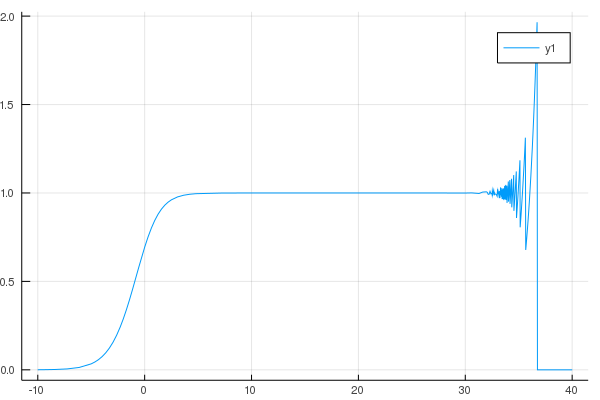
\includegraphics[width=\linewidth]{plot-jl}
  \end{minipage}
  \begin{minipage}{0.48\textwidth}
    \centering
    \caption{Float32}
    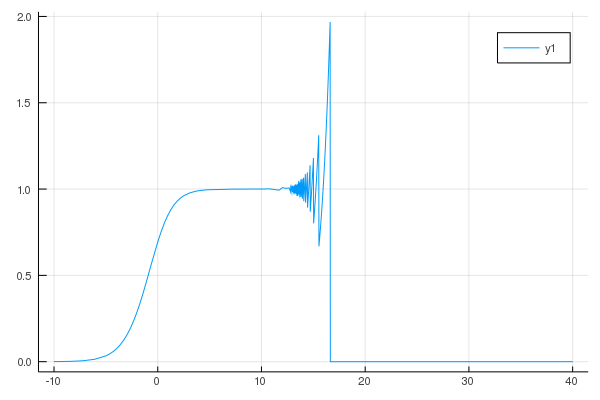
\includegraphics[width=\linewidth]{plot-jl32}
  \end{minipage}
\end{figure}
\subsection{Wnioski}
Analizując wykresy możemy zwrócić uwagę na szum pojawiający się w okolicach 30 (w przypadku arytmetyki Float64) oraz w okolicach 15 (w przypadku arytmetyki Float32). Po zaburzeniu wartości funkcji możemy zobaczyć na wykresie, że funkcja zbiega do zera. Porównując do wyliczonej wcześniej granicy zauważamy, że funkcja zamiast do zera powinna zbiegać do 1. Dzieje się to z tego powodu, że przy odpowiednich wartościach x wartość $e^{-x}$ jest na tyle mała, że pochłania ją 1 stojąca obok w równaniu. Następnie $\ln 1 = 0$ dlatego na wykresach widzimy nieścisłość z obliczonym wynikiem. Natomiast szum pojawia się z powodu niedokładnej wartości $e^{-x}$, przez co obliczony $\ln{(1 + e^{-x})}$ pomnożony przez bardzo dużą wartość $e^x$ daje nieprawidłowy wynik.



\section{Zadanie 3}
\subsection{Problem}
Problem polegał na przeanalizowaniu układu równań z macierzą kwadratową pod względem wskaźnika uwarunkowania zadania.

Należało wygenerować podanymi funkcjami macierz Hilberta oraz losową macierz stopnia n z zadanym współczynnikiem uwarunkowania. Następnie należało danym układem równań oraz znając x, obliczyć błąd względny.

Równanie: $Ax = b$ gdzie A jest daną macierzą oraz x=$(1,...,1)^{T}$. Macierz A miała zostać wygenerowana dwoma sposobami: A=$H_{n}$ gdzie $H_{n}$ jest macierzą Hilberta n-tego stopnia, a także A=$R_{n}$ gdzie $R_{n}$ jest losową macierza stopnia n z zadanym wskaźnikiem uwarunkowania c. Dane równanie należało rozwiązać dwoma sposobami: algorytm eliminacji Gaussa oraz odwrotnością (x=$A^{-1}b$).
\subsection{Wyniki}
\begin{center}
  \begin{tabular}{c|c|c|c|c}
  n & rząd & wskaźnik uwarunkowania & błąd względny - eliminacja Gaussa & błąd względny - inwersja \\
  \hline
  1 & 1 & 1.0 & 0.0 & 0.0\\
  2 & 2 & 19.28147006790397 & 4.227603326225575e-16 & 1.4043333874306803e-15\\
  3 & 3 & 524.0567775860644 & 6.312995352117186e-16 & 0.0\\
  4 & 4 & 15513.73873892924 & 2.1819484005185015e-15 & 4.547473508864641e-13\\
  5 & 5 & 476607.25024259434 & 8.99737540851766e-12 & 1.4911297558868156e-11\\
  6 & 6 & 1.4951058642254665e7 & 1.8866554820446764e-10 & 3.5689314550268525e-10\\
  7 & 7 & 4.75367356583129e8 & 1.8614175017153493e-8 & 1.231617281152939e-8\\
  8 & 8 & 1.5257575538060041e10 & 1.9217530132542664e-7 & 1.3503856270597747e-7\\
  9 & 9 & 4.931537564468762e11 & 5.09208671414057e-6 & 9.542631496737485e-6\\
  10 & 10 & 1.6024416992541715e13 & 5.508778842434553e-5 & 0.0002289249459044258\\
  11 & 10 & 5.222677939280335e14 & 0.005207147400142043 & 0.008849600746399502\\
  12 & 11 & 1.7514731907091464e16 & 0.1407902677571603 & 0.4039460424541017\\
  13 & 11 & 3.344143497338461e18 & 355.6363996139929 & 212.78257870436312\\
  14 & 11 & 6.200786263161444e17 & 3.5720053119125916 & 1.7744875020766255\\
  15 & 12 & 3.674392953467974e17 & 9.583022643862336 & 5.293638550842115\\
  16 & 12 & 7.865467778431645e17 & 11.968066192267113 & 10.846229140698135\\
  17 & 12 & 1.263684342666052e18 & 5.455797564762254 & 8.982730231514317\\
  18 & 12 & 2.2446309929189128e18 & 26.309523680963647 & 20.038300611698062\\
  19 & 13 & 6.471953976541591e18 & 22.59171398621913 & 15.359549749376397\\
  20 & 13 & 1.3553657908688225e18 & 5.658540758579833 & 7.992554067235351
  \end{tabular} \par
  \bigskip
  Macierz Hilberta
\end{center}

\begin{center}
  \begin{tabular}{c|c|c|c|c}
  n & rząd & wskaźnik uwarunkowania & błąd względny - eliminacja Gaussa & błąd względny - inwersja \\
  \hline
  5 & 5 & 1.0000000000000007 & 1.719950113979703e-16 & 7.021666937153402e-17\\
  5 & 5 & 10.000000000000002 & 4.0029660424867205e-16 & 4.124295487574583e-16\\
  5 & 5 & 999.9999999999674 & 1.6451392519176417e-14 & 1.6587787186393758e-14\\
  5 & 5 & 9.999999993245421e6 & 1.3099694661816385e-10 & 1.1998713733297805e-10\\
  5 & 5 & 1.0000771646871694e12 & 1.6010983905701105e-5 & 1.7933134877842953e-5\\
  5 & 4 & 5.446553640257849e15 & 0.18766764365058394 & 0.24125323832023476\\
  10 & 10 & 1.0000000000000009 & 2.016820280180126e-16 & 2.696722356863272e-16\\
  10 & 10 & 9.99999999999999 & 1.719950113979703e-16 & 2.6506211417561425e-16\\
  10 & 10 & 999.9999999999661 & 1.6461728708899027e-14 & 2.8024808959884797e-14\\
  10 & 10 & 9.999999997774877e6 & 1.330926308898944e-10 & 2.8143005263155073e-10\\
  10 & 10 & 9.999949580097267e11 & 3.19034565452155e-5 & 3.4313726712719984e-5\\
  10 & 9 & 5.281574117718314e15 & 0.772644442828404 & 0.6165109523719196\\
  20 & 20 & 1.0000000000000013 & 3.188872858294072e-16 & 5.827349035319211e-16\\
  20 & 20 & 10.000000000000007 & 4.4200263976433584e-16 & 6.483170143248366e-16\\
  20 & 20 & 999.9999999999692 & 2.445914805970674e-14 & 2.4931960849310002e-14\\
  20 & 20 & 9.999999999969393e6 & 9.054375192105989e-12 & 4.255035751619564e-11\\
  20 & 20 & 1.0000533837398918e12 & 1.4512647537820678e-6 & 4.264961199760036e-6\\
  20 & 19 & 6.986616543918112e15 & 0.12212396809790553 & 0.0905774221822397
  \end{tabular} \par
  \bigskip
  Macierz losowa
\end{center}
\subsection{Wnioski}
Analizując powyższe tabele wyników, możemy wywnioskować, że błąd względny jest związany z wskaźnikiem uwarunkowania. Dokładnie przyglądając sie wynikom widzimy, że duże wskaźniki uwarunkowania mają znaczny wpływ na wielkość błędu w ostatecznym wyniku. Możemy stwierdzić, że zadanie jest źle uwarunkowane, ponieważ patrząc i porównując wyniki możemy zauważyć, że błąd względny przy n = 20 biorąc pod uwagę macierz Hilberta dochodzi nawet do 700\%. Natomiast błędy w losowej macierzy wahają się między małymi wartościami czyli $10^{-16}$ a większymi czyli około 0.77 (77 \%), jednakże musimy brac pod uwage, to, że jest to macierz generowana losowo, dlatego błąd w pewnej mierze w tym przypadku zależy od wylosowanych wartości.



\section{Zadanie 4}
\subsection{Problem}
Zadanie polegało na przeanalizowaniu wielomianu wilkinsona. Za pomocą biblioteki Polynomials należało obliczyć 20 zer danego wielomianu. Obliczone pierwiastki sprawdzono obliczając |$P(z_{k})$|, |$p(z_{k})$| oraz |$z_{k} - k$| gdzie $z_{k}$ jest pierwiastkiem oraz $k \in {1, ... , 20}$ . Następnie należało przeprowadzić ten sam eksperyment zamieniając pierwszy współczynnik z -210 na -210-$2^{-23}$.
\subsection{Wyniki}
\begin{center}
  \begin{tabular}{c|c|c|c|c}
    k & |P($z_{k}$)| & |P($z_{k}$)| po zmianie & |p($z_{k}$)| & |p($z_{k}$)| po zmianie \\
    \hline
    1 & 36352.0 & 20992.0 & 38400.0 & 22016.0\\
    2 & 181760.0 & 349184.0 & 198144.0 & 365568.0 \\
    3 & 209408.0 & 2.221568e6 & 301568.0 & 2.295296e6 \\
    \vdots \qquad & \vdots \qquad & \vdots \qquad & \vdots \qquad & \vdots \qquad\\
    9 & 4.465326592e9 & 3.065575424e9 & 4.457859584e9 & 1.37174317056e11\\
    10 & 1.2707126784e10 & 7.143113638035824e9 & 1.2696907264e10 & 1.4912633816754019e12\\
    \vdots \qquad & \vdots \qquad & \vdots \qquad & \vdots \qquad & \vdots \qquad\\
    19 & 1.0278376162816e13 & 9.539424609817828e12 & 1.0278235656704e13 & 4.2525024879934694e17\\
    20 & 2.7462952745472e13 & 1.114453504512e13 & 2.7462788907008e13 & 1.3743733197249713e18
  \end{tabular}
\end{center}

\begin{center}
  \begin{tabular}{c|c|c}
    k & |$z_{k}$-k| & |$z_{k}$-k| po zmianie\\
    \hline
    1 & 3.0109248427834245e-13 & 1.6431300764452317e-13\\
    2 & 2.8318236644508943e-11 & 5.503730804434781e-11\\
    3 & 4.0790348876384996e-10 & 3.3965799062229962e-9\\
    \vdots \qquad & \vdots \qquad & \vdots \qquad \\
    10 & 0.009586957518274986 & 0.6519586830380406\\
    11 & 0.025022932909317674 & 1.1109180272716561\\
    \vdots \qquad & \vdots \qquad & \vdots \qquad \\
    19 & 0.0019098182994383706 & 2.004329444309949\\
    20 & 0.00019070876336257925 & 0.8469102151947894
  \end{tabular}
\end{center}
\subsection{Wnioski}
Patrząc na powyższe tabele możemy wywnioskować, że zadanie jest źle uwarunkowane. Możemy to stwierdzić na podstawie tego, że przy najmniejszych odchyleniach prawidłowego pierwiastka, które w tym przypadku wynoszą $10^{-13}$ możemy zaobserwować błąd w granicach 36 tysięcy. Każdy większy pierwiastek posiada większy błąd od poprzedniego. Skutkuje to tym, że wynik zamiast prawidłowego 0 odchyla się nawet o $10^{13}$. Po wprowadzeniu niewielkich zmian (dokładnie $2^{-23}$) do pierwszego współczynnika wielomiany możemy zaobserwować, że błąd prawidłowego wyniku z 36 tysięcy zmalał do 20 tysięcy, co nadal jest ogromną niedokładnością. Także możemy zauważyć, że po zmianach wielomian p(x) dla większych x jest obarczony większym błędem niż P(x) po zmianach, gdyż P(x) ma zbliżone odchylenie w obu przypadkach, czego nie można powiedzieć o p(x). Z tych powodów możemy stwierdzić, ze zadanie jest źle uwarunkowane, gdyż niewielkie zmiany w granicach $10^{-13}$ zmieniają ostateczny wynik o kilkadziesiąt tysięcy.



\section{Zadanie 5}
\subsection{Problem}
Zadanie polegało na wykonaniu eksperymentu wykonując funkcję modelu wzrostu populacji dla pewnych danych.

Model populacji:
\[p_{n+1} = p_{n} + rp_{n}(1 - p_{n}) \land n >= 0\]

Dane: $p_{0} = 0.01, r = 3, n = 40$.
\subsection{Wyniki}
\begin{center}
  \begin{tabular}{l|l|p{8cm}}
    & wykonanie pełnych n iteracji & wykonanie n iteracji z obcięciem cyfr po 3 miejscu po przecinku w 10tej iteracji\\
    \hline
    Float32 & 0.25860548 & 1.093568\\
    Float64 & 0.011611238029748606 & 0.7305550338104317
  \end{tabular}
\end{center}
Wykresy:
\begin{figure}[h]
  \begin{minipage}{0.48\textwidth}
    \centering
    \caption{Float64 - iteracja bez obcięcia}
    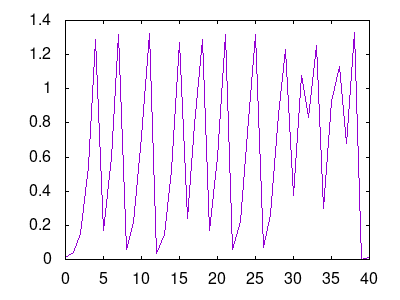
\includegraphics[width=\linewidth]{64}
  \end{minipage}
  \begin{minipage}{0.48\textwidth}
    \centering
    \caption{Float64 - iteracja z obcięciem}
    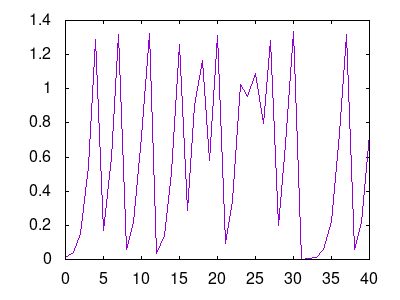
\includegraphics[width=\linewidth]{cut64}
  \end{minipage}
  \begin{minipage}{0.48\textwidth}
    \centering
    \caption{Float32 - iteracja bez obcięcia}
    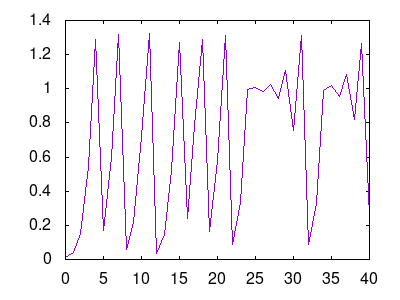
\includegraphics[width=\linewidth]{32}
  \end{minipage}
  \begin{minipage}{0.48\textwidth}
    \centering
    \caption{Float32 - iteracja z obcięciem}
    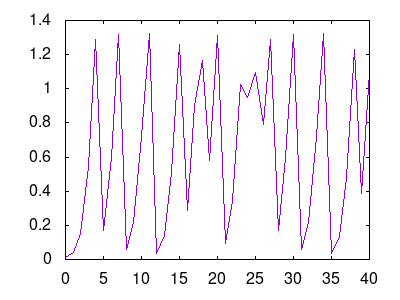
\includegraphics[width=\linewidth]{cut32}
  \end{minipage}
\end{figure}
\subsection{Wnioski}
Analizując powyższe wykresy możemy zauważyć, że uzyskane wartości są w miarę regularne. Po wprowadzeniu w 10tej iteracji ucięcia znaków po przecinku od 4 miejsca, możemy zauważyć różnicę w wynikach oraz delikatne zaburzenia w kolejnych krokach działania funkcji w przypadku Float64. Patrząc na Float32 dostaliśmy efekt zupełnie odwrotny, to znaczy po obcięciu otrzymaliśmy mniej zaburzeń na wykresie, lecz ostatecznie nadal mamy niedokłądne wyniki po n-tej iteracji. Dzieje się to dlatego, że w przypadku Float32 precyzja arytmetyki jest na tyle mała, że do momentu ucięcia cyfr po 4 miesju po przecinku wartosc posiadał już błąd spowodowany niewielką precyzją. Po ucięciu lekko zniwelowaliśmy ten błąd, lecz nadal szybko ujawniły się zaburzenia i błędy. W przypadku arytmetyki Float64 spotykamy się ze zjawiskiem gdy to precyzja arytmetyki jest na tyle wysoka, że przy iteracji, w której odcinami końcowe cyfry tracimy dokładność zamiast ją wzmocnić. Skutkiem tego jest szybsze zaburzenia w wynikach. W tabeli powyżej wykresami możemy zaobserwować wyniki po 40 iteracjach w obu eksperymentach. Widzimy, że wyniki różnią się od siebie w dużym stopni (porównując do 1), przez co możemy wywnioskować, że zaburzone iteracje są na tyle niewiarygodne, że otrzymane dane stają się bezuzyteczne w badaniu modelu populacji. Aby jak najlepiej zniwelować wystepujący tu problem należałoby użyć arytmetyki z jak największa precyzją, aby nieuniknione zaburzenia wystapiły w jak najpóźniejszej iteracji.

\section{Zadanie 6}
\subsection{Problem}
Problem polegał na przeanalizowaniu 40 iteracji ciągu rekurencyjnego: $x_{n+1} = x_{n}^2 + c \land n>=0$ dla różnych danych.

Dane:
\begin{enumerate}
\item $c = -2$ i $x_{0} = 1$
\item $c = -2$ i $x_{0} = 2$
\item $c = -2$ i $x_{0} = 1.99999999999999$
\item $c = -1$ i $x_{0} = 1$
\item $c = -1$ i $x_{0} = -1$
\item $c = -1$ i $x_{0} = 0.75$
\item $c = -1$ i $x_{0} = 0.25$
\end{enumerate}

\subsection{Wyniki}
\begin{figure}[H]
  \begin{minipage}{0.4\textwidth}
    \centering
    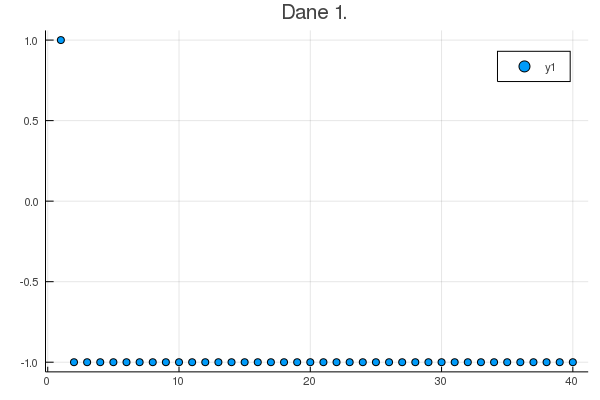
\includegraphics[width=\linewidth]{plot1}
  \end{minipage}
  \begin{minipage}{0.4\textwidth}
    \centering
    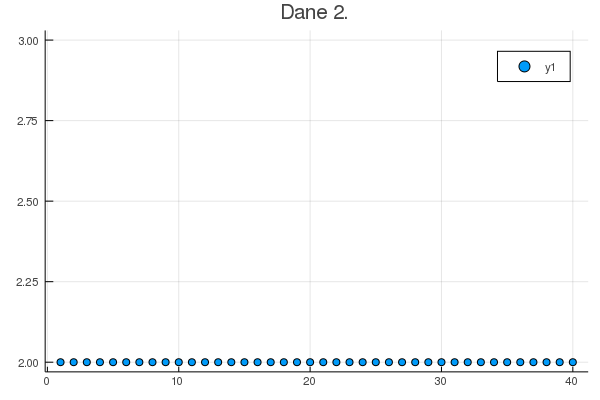
\includegraphics[width=\linewidth]{plot2}
  \end{minipage}
  \begin{minipage}{0.4\textwidth}
    \centering
    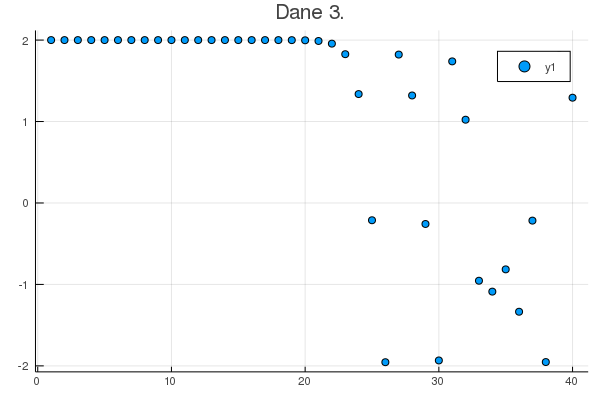
\includegraphics[width=\linewidth]{plot3}
  \end{minipage}
  \begin{minipage}{0.4\textwidth}
    \centering
    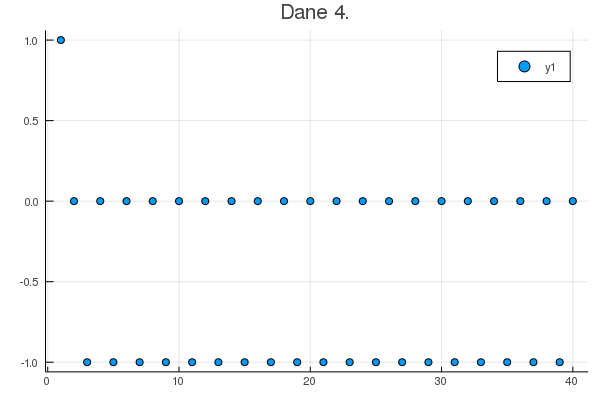
\includegraphics[width=\linewidth]{plot4}
  \end{minipage}
  \begin{minipage}{0.4\textwidth}
    \centering
    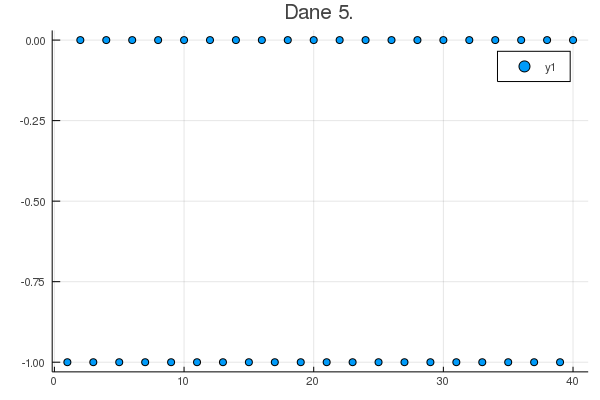
\includegraphics[width=\linewidth]{plot5}
  \end{minipage}
  \begin{minipage}{0.4\textwidth}
    \centering
    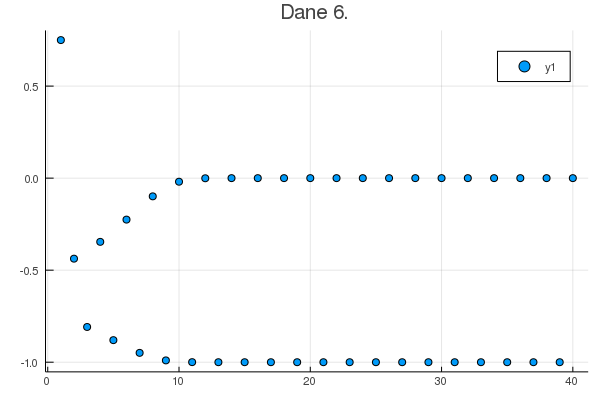
\includegraphics[width=\linewidth]{plot6}
  \end{minipage}
  \begin{minipage}{0.4\textwidth}
    \centering
    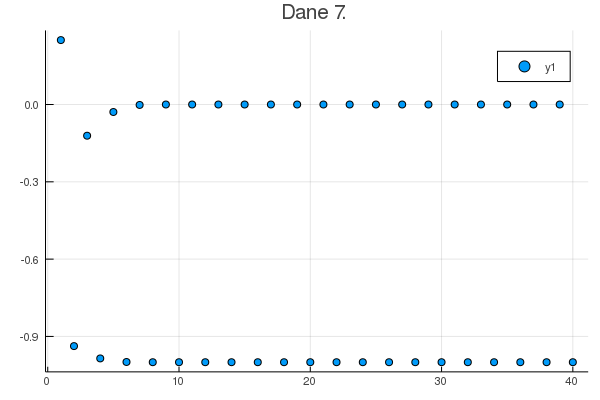
\includegraphics[width=\linewidth]{plot7}
  \end{minipage}
\end{figure}

\subsection{Wnioski}
Porównując podane dane z wykresami ciagów możemy zaobserwować, że przy c = -2 oraz x0 całkowitym ciąg jest prawie stały. Jedynie przy wartości x0 = 1.99999999999999 ciąg od pewnego momentu załamuje się i każdy punkt jest niregularny względem poprzedniego. W przypadku gdy stała c = -1 możemy zaobserwować, że ciagi mają w większości dwa punkty stałe na przemian a są nimi 0 oraz -1. Ciągi te różnią się jedynie poczatkowymi wartościami. Wywnioskować z tego można, że sposób dotarcia do punktów 0 oraz -1 danego ciagu jest zależny od punktu początkowego. Jednakże również wnioskujemy, że ciągi te zbiegają do liczb całkowitych, skutkiem czego możemy badać takie szeregi używając arytmetyki ze skończoną precyzją.
\end{document}
